% On découpe ce document complexe en plusieurs sous-fichiers séparés.
% Cela permettra notamment de réarranger les transparents facilement 
% lors de l'élaboration du document.

% La définition de la classe beamer avec tous les styles afférents

\RequirePackage{currfile} 

\documentclass{beamer}
%\documentclass{article}

%%%%%%%%%%%%%%%%%%%%%%%%%%%%%%%%%%%%%%%%%
% Beamer Presentation
% LaTeX Template
% Version 1.0 (10/11/12)
%
% This template has been downloaded from:
% http://www.LaTeXTemplates.com
%
% License:
% CC BY-NC-SA 3.0 (http://creativecommons.org/licenses/by-nc-sa/3.0/)
%
%%%%%%%%%%%%%%%%%%%%%%%%%%%%%%%%%%%%%%%%%

%----------------------------------------------------------------------------------------
%	PACKAGES AND THEMES
%----------------------------------------------------------------------------------------




\mode<presentation> {

% The Beamer class comes with a number of default slide themes
% which change the colors and layouts of slides. Below this is a list
% of all the themes, uncomment each in turn to see what they look like.

%\usetheme{default}
%\usetheme{AnnArbor} син+желт
%\usetheme{Antibes}
%\usetheme{Bergen}
%\usetheme{Berkeley}
%\usetheme{Berlin}
%\usetheme{Boadilla}
%\usetheme{CambridgeUS}
%\usetheme{Copenhagen}
%\usetheme{Darmstadt}
%\usetheme{Dresden}
%\usetheme{Frankfurt}
%\usetheme{Goettingen}
%\usetheme{Hannover}
%\usetheme{Ilmenau}
%\usetheme{JuanLesPins}
%\usetheme{Luebeck}
%\usetheme{Madrid}		
%\usetheme{Malmoe}
%\usetheme{Marburg}
%\usetheme{Montpellier}
%\usetheme{PaloAlto}%good
%\usetheme{Pittsburgh}
%\usetheme{Rochester}
%\usetheme{Singapore}
%\usetheme{Szeged}
\usetheme{Warsaw}

% As well as themes, the Beamer class has a number of color themes
% for any slide theme. Uncomment each of these in turn to see how it
% changes the colors of your current slide theme.

%\usecolortheme{albatross}
%\usecolortheme{beaver}
%\usecolortheme{beetle}
%\usecolortheme{crane}
%\usecolortheme{dolphin}
%\usecolortheme{dove}
%\usecolortheme{fly}
%\usecolortheme{lily}%!!!!!!!
%\usecolortheme{orchid}%!!!!!!!
%\usecolortheme{rose}
%\usecolortheme{seagull}
%\usecolortheme{seahorse}
\usecolortheme{whale}%!!!!!!!!!
%\usecolortheme{wolverine}

%\setbeamertemplate{footline} % To remove the footer line in all slides uncomment this line
%\setbeamertemplate{footline}[frame number] % To replace the footer line in all slides with a simple slide count uncomment this line

%\setbeamertemplate{navigation symbols}{} % To remove the navigation symbols from the bottom of all slides uncomment this line

\setbeamercovered{transparent} % Fait apparaître les animations en grisé (utile pour la conception, mais peut être commenté lors de la remise du document final)

% Pour utiliser une police à empattements partout
\usefonttheme{serif}

% Pour rajouter la numérotation des frames dans les pieds de page
\newcommand*\oldmacro{}%
\let\oldmacro\insertshorttitle%
\renewcommand*\insertshorttitle{%
  \oldmacro\hfill%
  \insertframenumber\,/\,\inserttotalframenumber}

}

\usepackage{graphicx} % Allows including images
\usepackage{booktabs} % Allows the use of \toprule, \midrule and \bottomrule in tables




% Les autres packages utiles  notamment pour le français, les accents ou Python
\usepackage{natbib}         % Pour la bibliographie
\usepackage{url}            % Pour citer les adresses web
\usepackage[T2A]{fontenc}
\usepackage[utf8]{inputenc}
\usepackage[russian,english,french]{babel}

\usepackage{numprint}       % Histoire que les chiffres soient bien

\usepackage{amsmath}        % La base pour les maths
\usepackage{mathrsfs}       % Quelques symboles supplémentaires
\usepackage{amssymb}        % encore des symboles.
\usepackage{amsfonts}       % Des fontes, eg pour \mathbb.

\usepackage{cancel}

%\usepackage[svgnames]{xcolor} % De la couleur

%%% Si jamais vous voulez changer de police: décommentez les trois 
%\usepackage{tgpagella}
%\usepackage{tgadventor}
%\usepackage{inconsolata}

%%% Pour L'utilisation de Python
\usepackage{minted}
\usemintedstyle{friendly}

\usepackage{graphicx} % inclusion des graphiques
\usepackage{wrapfig}  % Dessins dans le texte.

\usepackage{tikz}     % Un package pour les dessins (utilisé pour l'environnement {code})
\usepackage[framemethod=TikZ]{mdframed}

\usepackage{caption}
\captionsetup[figure]{font=small}


\usepackage{mathtools}
\usepackage{bbm}
\usepackage{dsfont}


\usepackage{pgfplots}
\usepackage{pgfplotstable}
% Les macros et raccourcis personnels
% Ce fichier contient toutes les macros que vous pouvez avoir envie de définir 
% si vous les utilisez plusieurs fois dans le document.

\PassOptionsToPackage{svgnames}{color}

% Un environnement pour bien présenter le code informatique
\newenvironment{code}{%
\begin{mdframed}[linecolor=green,innerrightmargin=30pt,innerleftmargin=30pt,
backgroundcolor=black!5,
skipabove=10pt,skipbelow=10pt,roundcorner=5pt,
splitbottomskip=6pt,splittopskip=12pt]
}{%
\end{mdframed}
}

% Un raccourci pour composer les unités correctement (en droit)
% Exemple: $v = 10\U{m.s^{-1}}$
\newcommand{\U}[1]{~\mathrm{#1}}

% Les guillemets \ofg{par exemple}
\newcommand{\ofg}[1]{\og{}#1\fg{}}

% Le d des dérivées doit être droit: \frac{\dd x}{\dd t}
\newcommand{\dd}{\text{d}}

% La dérivée temporelle, tellement courante en physique, avec les d droits
\newcommand{\ddt}[1]{\frac{\dd #1}{\dd t}}

% Des parenthèses, crochets et accolades qui s'adaptent automatiquement à la 
% taille de ce qu'il y a dedans
\newcommand{\pa}[1]{\left(#1\right)}
\newcommand{\pac}[1]{\left[#1\right]}
\newcommand{\paa}[1]{\left\{#1\right\}}

% Un raccourci pour écrire une constante
\newcommand{\cte}{\text{C}^{\text{te}}}

% Pour faire des indices en mode texte (comme les énergie potentielles)
\newcommand{\e}[1]{_{\text{#1}}}

% Le produit vectoriel a un nom bizarre:
\newcommand{\vectoriel}{\wedge}


% On définit le titre et l'auteur du document

% L'argument optionnel (entre crochets) donne le titre qui sera mis sur chaque slide
\title[ТВ и МС]{
\textbf{Лекции 2,~3}.  
\\
Эмпирическая функция распределения.
Функция риска.
}
\author{Лектор: Э.Ю. \textsc{Калимулина}} % Votre nom
% L'épreuve (car on n'a pas le droit de signaler sa provenance à un concours) (là encore, l'argument optionnel apparaît sur chaque slide)
\institute[TIPE]{Осенний семестр, 2022}
\date{курс \textsc{ТВ и МС}} 

% On démarre le document proprement dit
\begin{document}

% La page de titre et la table des matières
% Rien d'autre à faire qu'afficher le titre
\begin{frame}
\titlepage 
\end{frame}


% La table des matières utilise ce que vous donnez aux commandes \section et 
% \subsection tout au long de la présentation.
\begin{frame}
\frametitle{План лекции} 
\tableofcontents 
\end{frame}


% La première grande partie: introduction du sujet

\section{}


\section{Эмпирическая функция распределения.}
\subsection{Определение.}


\begin{frame}{Напоминание}
\begin{definition}
   Оценка (точечная) -- любая функция от элементов выборки 
   $$\hat{\theta}_n(\xi_1,..., \xi_n)$$ 
   со значениями в \textbf{параметрическом множестве} $\Theta$, 
которая каким-то образом аппроксимирует неизвестный параметр.

\end{definition}

\begin{definition}
Оценки (любые) в статистике называются \textbf{статистиками}.
Т.е. СТАТИСТИКА - любая оценка (как объект в МС).

\end{definition}



\end{frame}


\begin{frame}{Выборка}
В МС у нас есть результаты эксперимента. И нужно сделать вывод о свойствах самого эксперимента.  
$$
x_1,x_2, ...., x_n.
$$

Мы хотим по элементам выборки воссоздать (аппроксимировать) ф.р..

\end{frame}

\begin{frame}{Эмпирическая функция распределения. Определение.}


\begin{definition}
     \textbf{Эмпирическая функция распределения}:
     \begin{eqnarray}
         \hat{F_n}(x;~x_1,...,x_n) 
         \overset{\mathrm{def}}{=}
         \frac{1}{n}\sum_{i=1}^n
         %\mathbbm{1}
         \mathds{1}_{\{\xi_i \leqslant x \}}
     \end{eqnarray}
\end{definition}

 
эмпирическая ф.р.  (оценка)  зависит от вещественного числа $x$ и от элементов выборки

\end{frame}

\begin{frame}{Упорядоченная выборка:}
\begin{definition}
    Упорядоченная выборка:
    $$
    x_{(1)}~\leqslant~x_{(2)}~\leqslant~ ....~\leqslant~ x_{(n)}
    $$
    называется \textbf{вариационным рядом},
    \\
    а элементы этого ряда 
    $$x_{(k)}$$
    называются  \textbf{ $k$-ми порядковыми статистиками} (или статистиками порядка $k$).
\end{definition}

\end{frame}


\begin{frame}{График Э.Ф.Р.}

    
\end{frame}{}


\subsection{Несмещённость и состоятельность оценки $\hat{F_n}$}


\begin{frame}{Несмещённость и состоятельность оценки $\hat{F_n}$}
\begin{enumerate}
    \item 
    \textbf{Утверждение 1.~~}
 $$\forall x \in  \mathbb{R} ~~~\hat{F_n}(x;~ \xi_1,\xi_2,...,\xi_n)$$ --
есть
несмещенная оценка числа $F_{\xi_i}(x)$.
\end{enumerate}
Док-во:
\begin{align*}
\mathrm{\mathbf{E}} \hat{F_n}(x;~ \xi_1,\xi_2,...,\xi_n) & =
\\
\mathrm{\mathbf{E}} \bigg( \frac{1}{n}\sum_{i=1}^n
         %\mathbbm{1}
         \mathds{1}_{\{\xi_i \leqslant x \}} \mathrm{\mathbf{E}} \bigg) & =
\frac{1}{n} \mathrm{\mathbf{E}} \sum_{i=1}^n
         %\mathbbm{1}
         \mathds{1}_{\{\xi_i \leqslant x \}}  =
         \\
\frac{1}{n}  \sum_{i=1}^n
         %\mathbbm{1}
         \mathrm{\mathbf{E}} \mathds{1}_{\{\xi_i \leqslant x \}} & =
        \frac{1}{n}  \sum_{i=1}^n
         %\mathbbm{1}
         \mathrm{P} \{\xi_i \leqslant x \}  
         \overset{\mathrm{def}}{=}
         F_{\xi_i}(x).
\end{align*}


\end{frame}{}

\begin{frame}{Несмещённость и состоятельность оценки $\hat{F_n}$}
\begin{enumerate}[2]
    \item 
    \textbf{Утверждение 2.~~}
$$\forall x \in  \mathbb{R} ~~~\hat{F_n}(x;~ \xi_1,\xi_2,...,\xi_n)$$ --
есть
состоятельная оценка числа $F_{\xi_i}(x)$.
\end{enumerate}
Док-во (следствие (У)ЗБЧ):
$$
\mathrm{P} ( \mathds {1}_{ \{\xi_i \leqslant x\} }=1 ) =
\mathrm{P} ( \xi_i \leqslant x ) = F_{\xi_i} (x),
$$
\begin{align*}
\frac{ 
\mathds{1}_{ \{\xi_1 \leqslant x\} }
 ~ + ~...~+~
 \mathds{1}_{ \{\xi_n \leqslant x\} }
}
{n}
\xrightarrow[n \to \infty]{\text{п.н.}}
~~F_{\xi_i}.
\end{align*}

\end{frame}{}


\subsection{Теорема Гливенко – Кантелли.}


\begin{frame}{Теорема Гливенко – Кантелли}
$F_{\xi_i}(x)$ равномерно хорошо приближается $\hat{F_n}(x; \xi_1,...,\xi_n)$ не просто в одной точке, а на все числовой оси.

\begin{theorem}
\textbf{Теорема Гливенко -- Кантелли.}
\begin{eqnarray*}
    \mathrm{P}\bigg( \sup_{x \in  \mathbb{R}} 
    \big| \hat{F_n}(x; \xi_1,...,\xi_n) ~-~ F_{\xi}(x) \big|
    \xrightarrow[n \to \infty]{ } 0
    \bigg) =1.
\end{eqnarray*}
\end{theorem}
То есть для почти любого исхода который,
существует  в  пространстве $\Omega$, где определены  случайные величины $\xi_1,...,\xi_n$, фактически для почти любой
выборки, которая может породиться в рамках нашего эксперимента, не только эта разность близко к нулю, но даже супремум по всей
числовой
прямой.
\end{frame}

\subsection{Теорема Колмогорова}

\begin{frame}{Теорема Колмогорова}
\begin{theorem}
\textbf{Теорема Колмогорова.}
Пусть
$F_{\xi_i}$- непрерывная и пусть
\begin{eqnarray*}
\sqrt{n}D_n=
\sqrt{n}
\sup_{x \in  \mathbb{R}} 
    \big| \hat{F_n}(x; \xi_1,...,\xi_n) ~-~ F_{\xi}(x) \big|,
\end{eqnarray*}
тогда
\begin{eqnarray*}
\sqrt{n}D_n
    \xrightarrow[n \to \infty]{D}
    \eta:~~~~
    \\F_{\eta}(y)=
     \begin{cases}
      0 & \text{если $y \leqslant 0$ }\\
      \sum_{i=-\infty}^{\infty} (-1)^i e^{-2i^2y^2} & \text{если $y > 0$ },
    \end{cases}
\end{eqnarray*}
где $F_{\eta}(y)$ -- распределение Колмогорова.
\end{theorem}
\end{frame}

\section{Функция риска}

\begin{frame}{}
Еще  один способ сравнивать оценки точечные оценки.
Дано (как и всегда):
$$
x_1,...,x_n -- \text{выборка}
$$
$$
\xi_1,...,\xi_n -- \text{н.о.р.с.в} ~~\sim F_{\xi},
$$
$$
F_{\xi} \in \{F_{\theta} \}_{\theta \in \Theta}.
$$
Две оценки
$$
\hat{\theta_1}~~\text{и}~~\hat{\theta_2}.
$$
 Допустим, что они обе несмещенные и обе состоятельные. Какая лучше?
 
\end{frame}


\begin{frame}
\frametitle{Функция штрафа}
Рассмотрим разность:
$$
\hat{\theta}_n - \theta,
$$
где $\hat{\theta}_n$ -- оценка, а - $\theta$ -- истинное значение оцениваемого параметра. Сколько мы "заплатим" за неравенство нулю это разности?

~
~
\\
~


Введём некоторую функцию, называемую \textbf{функцией штрафа}  или \textbf{функцией потерь}:
 $$
 U(\cdot)
 $$


\end{frame}


\begin{frame}
\frametitle{Функция штрафа. Предположения.}

\textbf{Функция штрафа}  или \textbf{функция потерь}:
 $$
 U(\cdot)
 $$

Предположения:
\begin{enumerate}
    \item $$
U(0)=0,
$$
\item
$$
U(x)=U(-x) 
$$
- четная функция,
\item
$$
U(x)=U(-x) 
$$
монотонная.
\end{enumerate}




Примеры
$U(x)=x^2$, $U(x)=|x|$.
\end{frame}


\begin{frame}
\frametitle{Функция штрафа (для оценки)}
Естественно  в эту функцию
подставлять разность между оценкой и
неизвестным параметрам
$$
U(\hat{\theta}_n - \theta).
$$
Какой мы штраф заплатим за то, что оценка
ошиблась в какую-либо сторону.

\end{frame}

\begin{frame}
\frametitle{Функция риска}
Какой мы штраф заплатим за то, что оценка
ошиблась в какую-либо сторону.


Функция риска:
$$
\mathcal{R}_{\hat{\theta}_n}(\theta) = \mathrm{\mathbf{E}}U(\hat{\theta}_n - \theta),
$$
аргумент этой функции --  неизвестный параметр, который меняется
в рамках параметрического множества.



Примеры: квадратичная функция риска, или
абсолютная, и т.д.
\end{frame}


\begin{frame}
\frametitle{Функция риска}
Если оценка $\hat{\theta_n}$ --
несмещенная оценка параметра $\theta$, 
(то тогда параметр $\theta$ представляет собою математическое ожидание $\hat{\theta_n}$), 
и 
$$U(x)=x^2, $$

то 
$$
\mathcal{R}_{\hat{\theta}_n}(\theta) = \mathrm{\mathbf{D}}\hat{\theta}_n.
$$
\end{frame}



\begin{frame}{Картинка}

\end{frame}

\begin{frame}{Подходы}
\begin{enumerate}
    \item интегральный
    \item минимаксный
\end{enumerate}

\end{frame}

\begin{frame}{Интегральная оценка}
 $$
\int_{\Theta} \mathcal{R}_{\hat{\theta}_n}(\theta) d \theta 
\to \min_{\hat{\theta}_n}
$$
нас интересует  минимизация этого
интеграла  по
всем $\hat{\theta}_n$. 
\end{frame}

\begin{frame}{Миминимаксный (minimax)}
Минимаксный подход
$$
\max_{\theta \in \Theta} \mathcal{R}_{\hat{\theta}_n}(\theta)
\to \min_{\hat{\theta}_n}.
$$
\end{frame}



\begin{frame}
\frametitle{Пример}
Пусть у нас есть
$$
\xi_i \sim \mathcal{N}(\theta, \theta^2)
$$
Оцениваем параметр $\theta$ и считаем что:
$$
\hat{\theta}_n 
\pause
\in \{\mu_n 
\sum_{i=1}^n \xi_i\}
$$

Возьмем квадратичный риск
\begin{eqnarray*}
u(x)=x^2
\end{eqnarray*}
\end{frame}



\begin{frame}
\frametitle{Пример}
Квадратичная функция риска в нашем конкретном примере
$$
 \mathcal{R}_{\hat{\theta}_n}(\theta) =
 \mathrm{\mathbf{E}} (\mu_n \sum_{i=1}^n \xi_i
 - \theta  )^2
$$
\end{frame}

\begin{frame}
\frametitle{Пример}
\begin{eqnarray*}
 \mathcal{R}_{\hat{\theta}_n}(\theta) =
 \mathrm{\mathbf{E}} (\mu_n \sum_{i=1}^n \xi_i
 - \theta  )^2=
 \pause
 \\
 = \mathrm{\mathbf{E}} 
 \Bigg(\mu_n^2
 \pause
 (  \xi_1^2+...+\xi_n^2 +
 \pause
 \sum_{i \neq j} \xi_i \xi_j)
 \pause
 - 2 \mu_n  \theta   \sum_{i=1}^n \xi_i
 \pause
 + \theta^2
 \Bigg) =
 \pause
 \\
 \bigg/
 \mathrm{\mathbf{E}}\xi_i^2= \mathrm{\mathbf{D}}\xi_i+(\mathrm{\mathbf{E}} \xi_i)^2
 =
 \pause
 2 \theta^2,
 \\
 \sum_{i \neq j} \xi_i \xi_j =\theta^2
 \pause
 \bigg/
 \\
 =\mu_n^2 (2n \theta^2+n(n-1)\theta^2) \pause 
 - 2\mu_n \theta^2 n 
 \pause
 + \theta^2=
 \pause
 \\
 =\theta^2(\mu_n^2 2n - 2\mu_n  n +\mu_n^2n(n-1)+ 1)= \\
 \pause
 \theta^2(n(n+1)\mu_n^2 -2n \mu_n   + 1). 
\end{eqnarray*}
\end{frame}

\begin{frame}
\frametitle{Пример}
Окончательно получаем
\begin{align*}
 \mathcal{R}_{\hat{\theta}_n}(\theta) & =
 \\
 & =
 \theta^2(n(n+1)\mu_n^2 -2n \mu_n   + 1). 
\end{align*}
Квадратичная
функция риска может быть  равномерно минимизирована.
\pause
$$
\frac{2n}{2n(n+1)}=\frac{1}{n+1},
$$
Окончательный ответ:
$$
\mu_n=\frac{1}{n+1}.
$$
\end{frame}
%
\begin{frame}
\frametitle{Упражнение}
\textbf{Упражнение}. Примените минимаксный подход:
 $$
 \xi_i \sim Binom(1,\theta)
$$
$$
 a_n\sum_{i=1}^n+b_n, ~~\Theta=[0,1],
 $$
 $$
 u(x)=x^2.
 $$
\end{frame}

\begin{frame}{Упражнение}
    Минимаксной (имеющей наименьший максимум риска) в схеме Бернулли для квадратичного штрафа
является оценка \textit{Ходжеса—Лемана}:
$$
\hat{\theta}_n
= \overline{x}+
\frac{1}{1+\sqrt{x}}
\bigg(
{\frac{1}{2} - \overline{x}}
\bigg).
$$
\end{frame}
%
\begin{frame}{Задача}
    Разбор некоторых теоретических задач (на доске).
\end{frame}

\begin{frame}{Домашнее задание}
    См. на доске.
\end{frame}
%
%
%
%
%
%
%%
%
%
%
%
%





% La 2e partie: Le point de vue de la relativité restreinte
%% Titre de la partie
\section{Функция распределения}

%%%%%%%%%%%%%%%%%%%%%%%%%%%%%%%%%%%%%%%%%%%%%%%%
% Première diapo (avec des équations)
%%%%%%%%%%%%%%%%%%%%%%%%%%%%%%%%%%%%%%%%%%%%%%%%
\begin{frame}
\frametitle{Relativité Restreinte}
\framesubtitle{Dynamique relativiste}

\begin{itemize}
	\item	<1->	Nouvelle définition de la quantité de mouvement
	
	\onslide <2->{
	$$\vec{p} = \gamma\,m\vec{v}
	\qquad\text{avec}\qquad
	\gamma = \frac{1}{\sqrt{1 - \frac{v^2}{c^2}}}
	$$
	}
	
	\item	<3->	Avec les développements \ofg{classiques} et en posant 
	$u=1/r$, on en arrive à l'équation
	
	\onslide <4->{
	$$
	\onslide <5->
	\underbrace{
	\onslide <4->
	    \frac{\dd^2 u}{\dd \theta^2} + u = \frac{G M m\, E}{L^2\, c^2}
	\onslide <5->
	    }_{
	    \text{Partie usuelle}}
	\onslide <4->
	            + 
	\onslide <6->
	\underbrace{
	\onslide <4->	
	            \frac{\pa{G M m}^2}{L^2\, c^2}\, u
    \onslide <6->
               }_{\text{Partie relativiste}}
	$$
	}
	
	
\end{itemize}

\end{frame}


%%%%%%%%%%%%%%%%%%%%%%%%%%%%%%%%%%%%%%%%%%%%%%%%
% Deuxième diapo
%%%%%%%%%%%%%%%%%%%%%%%%%%%%%%%%%%%%%%%%%%%%%%%%
\begin{frame}
\frametitle{Relativité Restreinte}
\framesubtitle{Équation de l'ellipse}

\begin{itemize}
	\item	<1->	Équation différentielle remise en forme
	
	\onslide <2->{
	$$
	    \frac{\dd u}{\dd \theta} + B^2\, u = A 
	\onslide <3->
	        \quad \text{avec} \quad 
	            B  = \sqrt{1 - \pa{\frac{G M m}{L\, c}}^{\!\!2} }
	$$
	}
	
	\item	<4->	Équation de l'\ofg{ellipse}
	
	\onslide <5->
	$$
	u = \frac{A}{B^2} \pa{1 + e\cos{\pac{B\pa{\theta - \theta_0}}}}
	\onslide <6->
	\quad\text{soit}\quad
	r = \frac{p}{1+e\cos{\pac{B\pa{\theta - \theta_0}}}}
	$$
	
\end{itemize}

\end{frame}

%%%%%%%%%%%%%%%%%%%%%%%%%%%%%%%%%%%%%%%%%%%%%%%%
% Troisième diapo
%%%%%%%%%%%%%%%%%%%%%%%%%%%%%%%%%%%%%%%%%%%%%%%%
\begin{frame}
\frametitle{Relativité Restreinte}
\framesubtitle{Avance du périhélie}

\begin{itemize}
	\item	<1->	L'\ofg{ellipse} ne se referme pas sur elle-même du fait que $B\neq1$
	\item	<2->	Entre deux périhélies successifs, $\theta$ tourne de $2\pi +\delta$ où
	\onslide<3->
	$$
	\boxed{
    \delta = 2\pi\pa{\frac{1}{B} - 1}
    \approx \pi \pa{\frac{G\, M\, m}{L\, c}}^{\!\!2} 
    = \pi \, \frac{G M}{p\, c^2}
    = \pi\, \frac{G M}{a\, c^2\, \pa{1-e^2}}	
    }
	$$
	
	\item	<4-> Malheureusement, l'application numérique ne donne \ofg{que} 
	$7''$ d'arc par siècle...
	
\end{itemize}

\end{frame}


% La 3e partie: Le point de vue de la relativité générale
%% Le titre de la partie
\section{Математическое ожидание сл. в.}

%%%%%%%%%%%%%%%%%%%%%%%%%%%%%%%%%%%%%%%%%%%%%%%%
% Première diapo
%%%%%%%%%%%%%%%%%%%%%%%%%%%%%%%%%%%%%%%%%%%%%%%%

\begin{frame}
\frametitle{Relativité Générale}
\framesubtitle{Et zut...}

\begin{itemize}
	\item	<1->	Il n'y a plus guère de temps pour parler
	\item	<2->	Alors zou, on balance le résultat des calculs

$$
    \onslide<3->
    \underbrace{
    \onslide<2->    
    \frac{\dd^2 u}{\dd \theta^2} + u 
        = 
        \frac{G M m^2}{L^2} 
    \onslide<3->
    }_{\text{Partie classique}}
    \onslide<2->
    + 
    \onslide<3->
    \underbrace{
    \onslide<2->    
    \frac{3\, G M}{c^2}\, u^2
    \onslide<3->
    }_{\text{RG}}
    \onslide<2->
$$

	\item	<4->	Après avoir bien bossé, on obtient finalement
\onslide<4->
$$
	\boxed{
		\delta = 6\, \pi \, \frac{G M}{a\, c^2\pa{1-e^2}}
			}
$$

\end{itemize}

\end{frame}


%%%%%%%%%%%%%%%%%%%%%%%%%%%%%%%%%%%%%%%%%%%%%%%%
% Deuxième diapo: le code informatique impose un 
% environnement "fragile" pour la frame
%%%%%%%%%%%%%%%%%%%%%%%%%%%%%%%%%%%%%%%%%%%%%%%%

\begin{frame}[fragile]
\frametitle{
Дисперсиия величины $D \xi$}
\framesubtitle{Le code informatique}

\begin{code}
\begin{minted}[linenos]{python}

import scipy as sp
import scipy.optimize

def ma_fonction(x):
    return []

# À vous de remplir les choses adéquates...

\end{minted}
\end{code}
\end{frame}


% Conclusion
%% Le titre de la partie
\section{Дисперсия случайной величины}

%%%%%%%%%%%%%%%%%%%%%%%%%%%%%%%%%%%%%%%%%%%%%%%%
% Première diapo avec un exemple de tableau
%%%%%%%%%%%%%%%%%%%%%%%%%%%%%%%%%%%%%%%%%%%%%%%%
\begin{frame}
\frametitle{Дисперсия случайной величины}
\framesubtitle{Определение}
\theoremstyle{definition}
\begin{definition}{Дисперсией}
 величины $\xi$ (обозначается $D \xi$) называется величина
    $D\xi = E (\xi - E \xi)^2$
\end{definition}
\pause
\begin{definition}{}
Величина $\sigma = + \sqrt{ D\xi}$ называется стандартным отклонением значений
случайной величины $\xi$ от ее среднего значения $E\xi$.
\end{definition}
\end{frame}

\begin{frame}
\frametitle{Дисперсия случайной величины}
\framesubtitle{Свойства}
Поскольку
\begin{equation*}
    E(\xi - E\xi)^2 = E(\xi^2 - 2 \xi E\xi + (E \xi)^2 ) = \pause
    E\xi^2 - (E\xi) ^2 ,
\end{equation*}
\pause
то
\begin{equation*}
    \boxed{D \xi= E\xi^2 - (E\xi) ^2}.
\end{equation*}
\pause
\begin{equation*}
    \boxed{D \xi \geq 0}~~~\text{(из определения).}
\end{equation*}
\pause
\begin{equation*}
    \boxed{D (a+b\xi) =b^2 D\xi  }~~~\text{(из определения), где $a$, $b$ -  постоянные.}
\end{equation*}
\end{frame}

\begin{frame}
\frametitle{Ковариация случайных величин}
\framesubtitle{Определение}
Пусть $\xi$ и $\eta$ - две случайные величины. Тогда
\pause
\begin{eqnarray*}
    D(\xi + \eta) = E( \xi + \eta - E (\xi +  \eta ))^2 = 
    E( ( \xi - E \xi) + (\eta -  E \eta ) )^2 = \\
    = D  \xi + D \eta + 2
    \underbrace{
    E( \xi - E \xi)( \eta - E \eta)}_{ \pause cov (\xi, \eta) }.
\end{eqnarray*}
Величина $cov (\xi, \eta)$ называется ковариацией случайных величин $\xi$ и $\eta$.
\end{frame}

\begin{frame}
\frametitle{Корреляция случайных величин}
\framesubtitle{Определение, свойства.}
Если $\xi > 0$ и $\eta > 0 $, то величина
\pause
\begin{eqnarray*}
    \rho(\xi, \eta) = \frac{cov (\xi, \eta)}{\sqrt{\xi} \sqrt{\eta}}
\end{eqnarray*}
называется коэффициентом корреляции случайных величин $\xi$ и $\eta$.
\\
\\
\pause
Если $\rho(\xi, \eta) = \pm 1$, то 
$\eta = a \xi + b$, $(\xi, \eta)$ (линейно зависимы),
где $a > 0$, если $ \rho(\xi, \eta) = +1$, и $a < 0$, если $\rho(\xi, \eta) = -1$.
\end{frame}

\begin{frame}
\frametitle{Дисперсия}
\framesubtitle{Определение, свойства, ...}
Если $\xi$ и $\eta$ независимы, то независимы $\xi-E\xi$ и $\eta-E\eta$,  и по свойству 5) м. о.
\begin{eqnarray*}
cov(\xi, \eta) = E(\xi - E\xi) · E(\eta - E\eta) = 0.
\end{eqnarray*}
С учетом введенного обозначения для ковариации находим, что
\pause
\begin{eqnarray}\label{sum_of_dispers_0}
\boxed{
    D(\xi + \eta) = D(\xi) + D (\eta) + 2 cov (\xi , \eta).
    }
\end{eqnarray}
Если $\xi$ и $\eta$ независимы, то дисперсия суммы $\xi+\eta$ равна сумме дисперсий:
\begin{eqnarray}\label{sum_of_dispers}
\boxed{
D(\xi+\eta)=D\xi+ D\eta.
}
\end{eqnarray}

\end{frame}

\begin{frame}
\frametitle{Дисперсия}
\framesubtitle{Определение, свойства, ...}
Cвойство (\ref{sum_of_dispers}) остается выполненным и при меньшем предположении, нежели независимость $\xi$ и $\eta$: достаточно, чтобы величины $\xi$ и $\eta$ были некоррелированы, т. е. $cov(\xi , \eta) = 0$.
\end{frame}

\begin{frame}
\frametitle{Дисперсия}
\framesubtitle{Определение, свойства, ...}
\textbf{}{Замечание.}
Из некоррелированности $\xi$ и  $\eta$ вообще говоря, не следует их независимость.
\\
\\
\textbf{Пример}:  пусть случайная величина $\alpha$ принимает значения $0$, $\frac{\pi}{2}$ и $\pi$ с вероятностями $\frac{1}{3}$. Тогда $\xi=\sin \alpha$ и $\eta =\cos \alpha$
некоррелированы; в то же время они не только не независимы относительно вероятности $P$:
\begin{eqnarray*}
P(\eta =1, \xi=1) = 0 \neq  1/9 = P(\eta =1) P(\xi=1)
\end{eqnarray*}
Более того, $\xi$ и  $\eta$ - функционально зависимы: 
\begin{eqnarray*}
\eta ^ 2 + \xi ^ 2 = 1.
\end{eqnarray*}
\end{frame}

\begin{frame}
\frametitle{Дисперсия}
\framesubtitle{Определение, свойства, ...}
\textbf{}{Замечание.}
Из некоррелированности $\xi$ и  $\eta$ вообще говоря, не следует их независимость.
\\
\\
\textbf{Пример}:  пусть случайная величина $\alpha$ принимает значения $0$, $\frac{\pi}{2}$ и $\pi$ с вероятностями $\frac{1}{3}$. Тогда $\xi=\sin \alpha$ и $\eta =\cos \alpha$
некоррелированы; в то же время они не только не независимы относительно вероятности $P$:
\begin{eqnarray*}
P(\eta =1, \xi=1) = 0 \neq  1/9 = P(\eta =1) P(\xi=1)
\end{eqnarray*}
Более того, $\xi$ и  $\eta$ - функционально зависимы: 
\begin{eqnarray*}
\eta ^ 2 + \xi ^ 2 = 1.
\end{eqnarray*}
\end{frame}

\begin{frame}
\frametitle{Дисперсия}
\framesubtitle{Определение, свойства, ...}
Свойства (\ref{sum_of_dispers_0}) и (\ref{sum_of_dispers}) для $\xi_1, \cdots, \xi_n$:
\begin{eqnarray}
\boxed{
    D(\xi_1 + \dots + \xi_n) = D(\xi_1) + \dots + D (\xi_n) + 2 \sum_{i>j} cov (\xi_i , \xi_j).
    }
\end{eqnarray}
\pause
Если $\xi_1, \dots, \xi_n$ попарно независимы (попарно некоррелированы):
\begin{eqnarray}\label{sum_of_dispers}
\boxed{
D \left(\sum_{i=1}^n  \xi_i \right)= \sum_{i=1}^n D\xi_i.
}
\end{eqnarray}
\end{frame}

\begin{frame}
\frametitle{Дисперсия}
\framesubtitle{Определение, свойства, ...}
Свойства (\ref{sum_of_dispers_0}) и (\ref{sum_of_dispers}) для $\xi_1, \cdots, \xi_n$:
\begin{eqnarray}
\boxed{
    D(\xi_1 + \dots + \xi_n) = D(\xi_1) + \dots + D (\xi_n) + 2 \sum_{i>j} cov (\xi_i , \xi_j).
    }
\end{eqnarray}
\pause
Если $\xi_1, \dots, \xi_n$ попарно независимы (попарно некоррелированы):
\begin{eqnarray}\label{sum_of_dispers}
\boxed{
D \left(\sum_{i=1}^n  \xi_i \right)= \sum_{i=1}^n D\xi_i.
}
\end{eqnarray}
\end{frame}




% Les slides d'exemples 
% (à commenter si bien sûr vous n'en voulez pas... 
% ils sont juste là pour servir d'exemples de base)
%\section{Примеры}
%\begin{frame}
\frametitle{Примеры}
\framesubtitle{}

\begin{itemize}
	\item	<1-> $\xi$ - бернуллиевская сл.в., принимающая два значения $1$ и $0$ с вероятностями $p$ и $q$:
	<2->
	\begin{equation*}
	   D\xi= E(\xi - E\xi)^2=E(\xi - p)^2=(1-p)^2p+p^2q=pq.
	\end{equation*}
	\item   <3-> $\Rightarrow$ если $\xi_1, ..., \xi_n$ - н.о.р берн. сл.в., $S_n=\xi_1 +...+\xi_n$, то 
$DS_n=npq$.
\end{itemize}

\end{frame}

\begin{frame}
\frametitle{Пример}
\framesubtitle{Оптимальное линейное оценивание}

\begin{itemize}
	\item $\xi$ и $\eta$, наблюдается лишь сл.в. $\xi$, предполагается, что $\xi$ и $\eta$ - коррелированы. \pause $f=f(\xi)$ от $\xi$ называется \textit{оценкой} для $\eta$. \pause $f^*=f^*(\xi)$ от $\xi$  -  \textit{оптимальная в среднеквадратическом смысле оценка} для $\eta$, если:
		\begin{equation*}
	   E(\eta - f^*(\xi))^2= \inf_f E(\eta - f(\xi))^2.
	\end{equation*}
	\pause
	Найдём оптимальную оценку в классе линейных оценок
$\lambda(\xi) = a + b \xi$: $\Rightarrow (*)$
\end{itemize}

\end{frame}


\begin{frame}
\frametitle{Пример}
\framesubtitle{Оптимальное линейное оценивание}
$(*)$
\pause $g(a,b)=M(\eta - (a + b\xi))^2,$
\begin{eqnarray*}
\pause \frac{\partial g(a,b)}{\partial a}=-2M(\eta - (a + b\xi)),
\\
\pause \frac{\partial g(a,b)}{\partial b}=-2M \left[ (\eta - (a + b\xi))\xi \right],
\end{eqnarray*}
$\Rightarrow$ \pause
   \boxed{
   $$\lambda^*(\xi) = E \eta + \frac{cov (\xi, \eta)}{D \eta} (\xi - E\xi)$$%.
}
\pause
\\
Cреднеквадратическая ошибка оценивания равна:
   \boxed{
   $$\Delta^*=E( \eta -\lambda^*(\xi))^2 = D \eta( 1 - \rho^2 (\xi , \eta)$$%.
}
\end{frame}

%\begin{frame}
\frametitle{Exemples}
\framesubtitle{Apparition d'une figure}

On peut aussi mettre du texte brut avant apparition d'une figure

\visible<2-> {% On n'utilise pas "\onslide" ici car on ne peut pas régler le niveau de transparence de la figure
\begin{center}
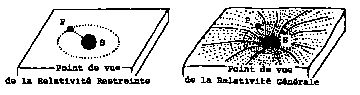
\includegraphics[width=0.5\linewidth]{figures/Fig02}
\end{center}
} % NB: \visible rend visible son argument, c'est-à-dire qu'il faut mettre ce 
  % qu'on veut rendre visible entre accolades par la suite contrairement à \onslide
  % qui joue le rôle d'une bascule.

\onslide<3->
Et le texte qui suit

\end{frame}

%\begin{frame}[fragile]
\frametitle{Exemples}
\framesubtitle{Apparition d'une équation en plusieurs temps}

L'idée est d'utiliser \verb|\onslide| pour faire apparaître les morceaux uns à 
uns. Cela correspond à des bascules qui imposent le comportement de tout ce qui 
suit jusqu'au prochain \verb|\onslide|. Par exemple, avec votre vieil ami 
l'oscillateur harmonique

$$
\onslide<3>
	1\times
\onslide<2->
	\frac{\dd^2\theta}{\dd t^2} + 
\onslide<4>
	\overbrace{
\onslide<2-> 
	\frac{g}{\ell}
\onslide<4>
	}^{={\omega_0}^2}
\onslide<2-> 
	\times\theta
	=
\onslide<5>
	\overbrace{
\onslide<2-> 
	A
\onslide<5>
	}^{=\theta\e{éq}\times{\omega_0}^2}
\onslide<2-> 
$$

\onslide<6->
Le mieux est d'écrire l'équation voulue en une fois avec tous les rajouts et de découper ensuite. Par exemple ici, ce serait

\onslide<7->
$$
	1\times
	\frac{\dd^2\theta}{\dd t^2} + 
	\overbrace{  	\frac{g}{\ell}  	}^{={\omega_0}^2}
	\times\theta	=
	\overbrace{	A	}^{=\theta\e{éq}\times{\omega_0}^2}
$$


\end{frame}


\end{document}


